\section{Specification}
This section considers the formal project plan that was created for the development of this projects, and the decisions on how it was structured. This phase of the project came after the specific project goals were identified during research (See \ref{ressummary}) and act's to create a development plan based on achieving these goals.

Each of the subsections then focus on one particular aspect of that planning.

\subsection{Development Methodology} \label{devmet}
PXP as introduced in the research phase \ref{otherresearch} was selected for its well defined (extensively documented) agile based methodology that was well suited to a single-person development team. Agile in general though, was selected over a waterfall technique to allow user feedback to drive design and development which was planned to be often collected.
As is a fundamental principle of agile this methodology was adapted to the project at hand (And the students work style) with some main changes and additions being:
\begin{itemize}
    \item Allow refactoring to be raised at any point, also allow grouping of similar user stories to be refactored together. Allowed fixing problems before they became too big and interlinked.
    \item MoSCoW and Cost factors agile ceremonies were applied to the project’s user stories. Allowed better planning and time management.
    \item Instead of tasks created from user stories, user stories themselves are treated like tasks with any non-user story work labelled as tasks instead and treated the same as stories. Done to lower duplication of information.
    \item No automated testing. This was a decision that was retroactively added here after prototyping during the design phase (See \ref{automatedtests}). The justification for this controversial change is covered there but in summary, It was found that Graphics development is fairly tricky to automate the testing of as the large majority of testing is completely visual and subject to changes.
    \item Reworked development process in general to better fit the students workflow. See \ref{scheduling} and \ref{devflow} for specific details
\end{itemize}

To see the resultant development flow with these changes in action see Section \ref{implementation}.

\subsection{Requirements Gathering}
With the goals that the developed application needs to achieve set as per the research phase (See \ref{ressummary})- The next step was to create a concrete plan on what exact requirements / features would contribute towards achieving those goals. To do that, two main ideas were identified by the student.

The first idea was to conduct Interviews with individuals who commonly use visualization tools or do general data science work. This would provide key insight into what real users of visualization technology think is key for a successful application to have. These requirements would constitute the first phase of the project and set a strong start to either a waterfall type methodology or an agile project.
But there were a couple of downsides that cancelled out this idea at that time:
\begin{itemize}
    \item With no initial product to focus insight into actionable requirements- the interview process is more likely to return conflicting or infeasible requirements.
    \item It might be difficult to offer insight that is not generic for the same reasons. Application should plot data vs Application should do it like this instead of like this. With the latter insight being much more valued.
    \item Time and access to experts is very valuable and needs extensive preparation. It is important to make the most of it, which the student didn’t feel like they could do at that time.
\end{itemize}

The next idea to identify requirements was one which was inspired by the development methodology chosen to be followed by the student in section \ref{devmet}, PXP, the methodology in question, describes the process for a developer to stand in for the client if the client is unavailable for planning. So, The student took on the role of the client to create a client brief using the insight gained during the research phase. This had a number of key advantages listed as follows:

\begin{itemize}
    \item Minimal Preparation and much faster compared to planning and hosting an interview.
    \item Can take advantage of previous research into market competitors to inspire requirements.
    \item With the "Client" also being the developer it is possible to think more deeply about how possible the stories are and how well they fit together.
\end{itemize}

With this technique, a planning stage was ran and a requirements brief was created. This brief can be read in full in Appendix A but in short, creates a written source document describing the minimum simplest application that would need to be created. It was considered that only a minimal version of the application should be planned at the beginning with further improvements then coming in a more agile way through user testing and analysis by the student based on how the project is progressing.

But the main reason to have created this brief instead of just skipping to creating user stories directly was to have a consistent main source from where user stories were pulled from and were focused on meeting the goals set during the research phase (See \ref{ressummary}).

With a brief set, the next step was to extract user stories (formal requirements) from the brief. Those initial user stories all formed the MVP (minimum viable product) feature set which were scheduled as further covered in section \ref{scheduling}. The specific extracted user stories and their analysis follow as so (See Table. \ref{req1})

\begin{table*}[t]
    \begin{tabular}{ | l | l | l | }
        \hline
        ID & Title                                                                                                               & Estimate (Relative) \\
        \hline
        1  & As a User, I want to be able to import a dataset into the application to graph it in a 3 dimension scatterplot      & 3                   \\
        \hline
        2  & As a User, I want to be able to navigate around the generated graph in 3D space while having the axis stay accurate & 6                   \\
        \hline
        3  & As a User, I want to be able to view a scatterplot of data set against an axis with accurate scales                 & 5                   \\
        \hline
        5  & As a User, I want to move the 3D view of the scatterplot in 3D using on screen controls                             & 3                   \\
        \hline
        6  & As a User, I want to be able to zoom in and out of the 3D Scatterplot                                               & 10                  \\
        \hline
        7  & As a User, I want to be able to rotate the 3D Scatterplot around all 3D axis individually                           & 5                   \\
        \hline
        8  & As a User, I want the application to have easy to use on screen controls for interacting with the application       & 3                   \\
        \hline
        9  & As a User, I want to be able to access the application on landscape screens of different sizes                      & 2                   \\
        \hline
        10 & As a User, I want to be able to view instructions within the application on how to use the application              & 2                   \\
        \hline
        11 & As a User, I want all interactable parts of the Application to be visible at all times                              & 1                   \\
        \hline
    \end{tabular}
    \caption{Requirements Gathering \#1 User Stories, MVP Feature Set}
    \label{req1}
\end{table*}

\subsection{Project Management Tools}
A number of tools and services were employed in the process to allow the organization and techniques mentioned to be applied. Those consisted of the following:

\subsubsection{Git, Version Control}
A version control tool is an important tool for controlling and recording changes to a codebase.
Git specifically though was chosen due to the student having previous experience, and to allow GitHub to be used within the project for it's supporting tools (See \ref{github} and \ref{github2}).

\subsubsection{GitHub, Cloud Code Repositary} \label{github}
Github is a cloud host for git repositories with additional extensive tooling to support all aspects of a software development project. The student has had extensive experience with this platform thus it was chosen for this project to minimize learning downtime. Alternatives such as Bitbucket and GitLab also exist but did not offer any further advantages that the student considered worth the learning downtime.

\subsubsection{GitHub Issues and Projects, Organizing Backlog and managing stories} \label{github2}
GitHub also has integrated issues and project views for organizing and tracking stories. An alternative would not have been as tightly integrated with the code repository.

\subsection{Scheduling} \label{scheduling}
With a backlog of user stories ready the next step was to combine similar stories into feature sets. Feature sets were then given a deadline on when all of their user stories should be completed.
This would allow then the student to pick the most urgent Feature Set to focus on.

Once a Feature set was picked, each user story and task within was analyzed and given a development time cost and importance to the project. With this, a prioritized backlog was created that was split among the maximum iterations/sprints that would fit into the Feature set's time frame with a consideration for the students iteration velocity. On the off chance that there wasn't enough time to complete all stories and tasks, the student would re-analyze what stories and tasks could be dropped due to time constraints.

Having feature sets allowed the student to put into perspective what are the major additions to the application and if there was enough time to fully develop those additions.

The specifics of when each feature sets deadline was set and how it changed can be seen on a sprint by sprint basis in the implementation section (See \ref{implementation}).

\subsection{Development Flow} \label{devflow}
\begin{figure}
    \centering
    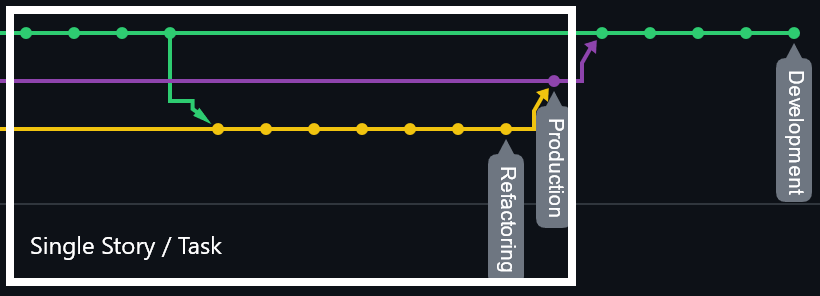
\includegraphics[width=1\columnwidth]{author-files/figures/SingleStoryPath2.png}
    \caption{Development Timeline of a Single Story}
    \label{fig:singlestory}
\end{figure}

Development followed a predefined process (See Figure \ref{fig:singlestory}) where a user story or task was picked to be developed. Once the student has finished developing the one or more tasks, the student would then push the code to the refactor branch where it would be organized and possibly reworked to follow better practices. This process allowed the student to move fast and encounter obstacles in implementation much more quickly, which minimized the risks of large roadblocks knocking the schedule out of balance. But once the feature was reworked to a sufficient standard with bugs fixed, it would then be fully tested and only then would be pushed to the final Production branch, which was build and publicly hosted.
This process helped ensure that any code committed to production was vetted and would be unlikely to cause unexpected issues. It also allowed the student to always have a safe version of the application for demos and user testing without having to worry about what work was done before hand.
The production version is then pushed to the development branch and the cycle repeats.


